

\chapter{Heuristic optimization}


%---------------------------------------------
%---------------------------------------------
%---------------------------------------------

\section{Introduction}

This chapter present different classes used for optimizing
functions with an approach different from the  refernce method : least square matching.
Compared to least square matching, this method has pro and cons. The inconvenient of this approach :

\begin{itemize}
   \item  slower 
   \item  dont extand to high dimension (for now in \PPP , limited to $5$);
\end{itemize}

By the way,  in some context this approach can have some advantage :

\begin{itemize}
   \item  simpler , because the user has only to give the function to minimize;

   \item  more general (for low dimension) because the
          the function has not to be  derivable, nor the be the sum of elementary linear observation

   \item  someway more robust, are we are "sure" of converging to a local minima.
\end{itemize}


%---------------------------------------------
%---------------------------------------------
%---------------------------------------------
\section{Disrcret optimization with class {\tt cOptimByStep}}


\label{HeurOpt:OBS}

%----------------------------------------------------------------------------

\subsection{Mathematicall formalization}

\label{Disc:Opt:Math}

\begin{figure}
\centering
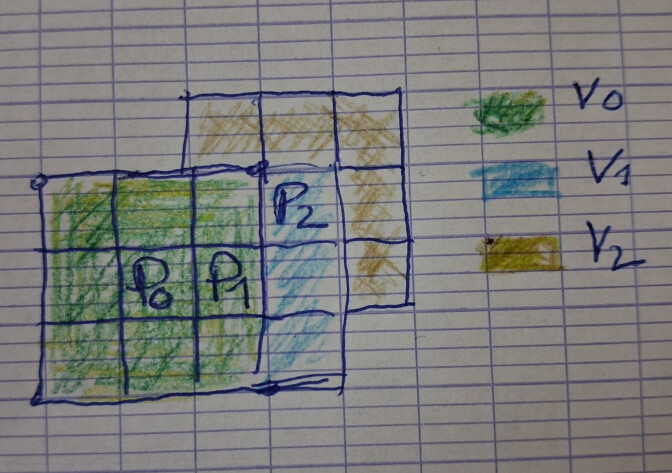
\includegraphics[width=8cm]{Programmer/ImagesProg/LocMin.jpg}
\caption{Illustration of restritcted values computed}
\label{fig:Path:HeuristikOpt}
\end{figure}

The classes of file {\tt MMVII\_HeuristikOpt} , can be used to find a
local extrema  of a function $F : \RR^D \rightarrow \RR$ by sucessive discrete resarch
at decreasing scale.


The algorithm used for research an extrema at a given scale/step $\Delta $ is quite simple :

\begin{itemize}
    \item let $N_d$ be the set of points $P$ of  $\ZZ^D$ such that $|P|_{\infty} \leq 1$ 
           and $|P|_{1} \leq d$ ; i.e. for $D=2$, $N_1$ and $N_2$ are the 
           well known $4$ and $8$ neighboors;


    \item  let $P$ be the current point  and set
           let $N_{d,\Delta}(P) = \{P+\Delta Q : Q \in N_d\}$
          
    \item compute the extrema $\overline P$ of $F$ in   $N_{d,\Delta}(P)$ ;
    \item if $P$ equal  $\overline P$ end at this step, else continue and set $P= \overline P$;
\end{itemize}

By the way, a value added of using \PPP's implementation is that
the method take care to limit the number of evaluation. At first 
iteration all the neighboor are explored, but at next iteration, the algorithm
avoid the point that have been explored at previous step.  Figure ~\ref{fig:Path:HeuristikOpt} :
illustrates an example, with $D=2$ on


\begin{itemize}
    \item  at first step, $F$ is evaluated for the $9$  points $V_0$ arround $P_0$ ;
    \item  at second step, $F$ is evaluated on  $3$  points $V_1$ arround $P_1$ were not already in $V_0$;
    \item  at second step, $F$ is evaluated on  $5$  points $V_2$ arround $P_2$ were not already in $V_1$.
\end{itemize}

Once an extrema is found at given scale $\Delta$ , the next iteration is done
at step $\Delta * \rho$ . This is done untill $\Delta < \epsilon$.

%----------------------------------------------------------------------------

\subsection{Maintener's point of view}

To implemant efficiently this optimisation,  a static dictionnary  $M$ is computed, that for
each direction give the list of next direction. For example in dimension $2$, using Freeman
code \footnote{https://de.wikipedia.org/wiki/Freeman-Code} , we will have $M[0]= {7,0,1} , M[1]={7,0,1,2,3}$.
The computation is made :

\begin{itemize}
   \item  {\tt AllocNeighbourhood<D>(d)} computes  $N_d$;
   \item  {\tt VLNeighOptim<D>(d)} computes the mapping $M$;
\end{itemize}


%----------------------------------------------------------------------------

\subsection{Programmer point of view}

The programmer control the parameters of \ref{Disc:Opt:Math} with two functions :
the constructor {\tt cOptimByStep}  and the method {\tt Optim}.

The constructor {\tt cOptimByStep}  takes $4$ parameters :

\begin{itemize}
   \item first is the function $F$  to miminize/maximize, it is a mapping {\tt cDataMapping<tREAL8,D,1> };
   \item a boolean indicating if we minimize (true) or maximize;
   \item a threshold $T$ that stop the computation if the distance to initial point is over $T$
         (some guardrail, not used so often \dots) ;
   \item the value $d$ used in $N_d$, default is $d=D$.
\end{itemize}

The method {\tt Optim} takes $4$ parameters ;

\begin{itemize}
   \item the initial point of $\RR^D$;
   \item the initial step $\Delta_0$ ;
   \item the value $\epsilon$ fixing when stop the computation (i.e. when $\Delta < \epsilon$);
   \item the ratio $\rho$ for evolution of $\Delta$ such that $\Delta_{k+1} = \rho * \Delta_k$.
\end{itemize}

%----------------------------------------------------------------------------

\subsection{Example of use}

\begin{figure}
\centering
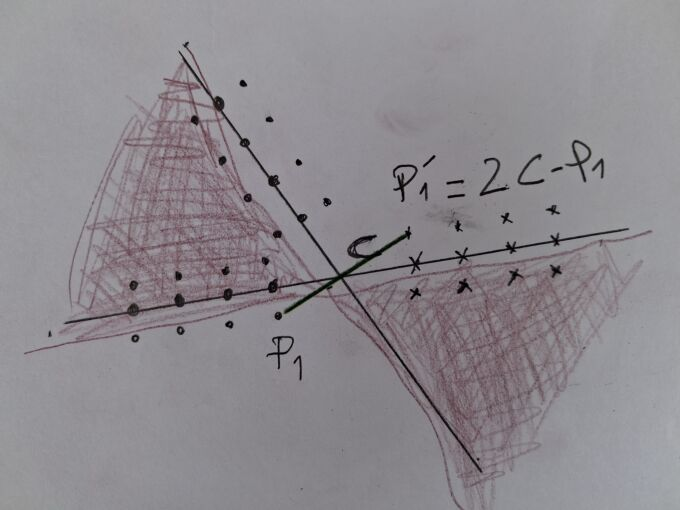
\includegraphics[width=8cm]{Programmer/ImagesProg/OptIm.jpg}
\caption{Using {\tt cOptimByStep} for optimizing the center of symetry on an image, dot points
         are $P_i$ and cross point are their symetric}
\label{fig:OptIm:HeuristikOpt}
\end{figure}

The \PPP code use this approach in several case when optimization the fitting
of parametric  model (primitive) on a image. For example, it used to refine
the position of a local symetry center. Illustrated  by figure~\ref{fig:OptIm:HeuristikOpt},
we describe how the center of check-board target\footnote{the symetry optimization can be
used in other context,  this the parameter initialization that is specific to check-board}
 are optimized using this approach:

\begin{itemize}
   \item we start from an initial centerl $C$ and an approximative detection of the $2$
         segment;

   \item we select a number of point $P_k$ arround one side of these $2$ segment (in fact any set of point
         should comply with symetry criteria, the fact of taking point close to segment is 
         justied because this the point that are very sensitive to symetry criteria, and limiting
         the number of point make computation more efficient);

   \item for a given symetry center $C$, the symetric of $P_k$ is $2*C-P_k$, if $C$ is the
         symetry center we should have $\forall k : I(P_k) = I(2*C-P_k)$ ;

   \item we use {\tt cOptimByStep<2>} to find the symetry center $C$ that minimize the function
         $Sym$ of equation~\ref{ImSym:HeuristikOpt}.
\end{itemize}

\begin{equation}
   Sym(C) = \sum_k |I(P_k) = I(2*C-P_k)| \label{ImSym:HeuristikOpt}
\end{equation}

%----------------------------------------------------------------------------------------
%----------------------------------------------------------------------------------------
%----------------------------------------------------------------------------------------

\section{Sampling the sphere, and projective sphere}

\label{Sec:Samp:Sphere}

%----------------------------------------------------------------------------
\subsection{Introduction}

In photogrammetry-metrology there is different case where we need to
optimize a function on one of the following manifold $\MM$:

\begin{itemize}
   \item on the sphere $\SPH^N$ ;
   \item on the projective sphere  $\RP^N$ (see~\ref{HeurOpt:ProjSph})
   \item on cartesian product of previous spaces $\SPH^N \times \SPH^Q $ ,  
         $\SPH^N \times \RP^Q $, $\RP^N \times \RP^Q $
\end{itemize}

Before doing some local optimization with the help of tools
described in~\ref{HeurOpt:OBS}, we need to have a point closed
enough to the globak minimal.  As the previous $\MM$  are
bounded manifold we know that with sufficiently high number  of samples,
we can be as close as we want to any point $\MM$ 
\footnote{\emph{Pedantically} speaking, because $\MM$ is compact}.

So the tools presented in this section allow to compute an arbirtrary
dense sampling of $\SPH^N$. This sampling are not perfectly regular,
and by the way we know that for $N>2$ there is only few regular 
sampling, \footnote{see for example https://en.wikipedia.org/wiki/Platonic\_solid
for the well known case of $\SPH^2$}.

%----------------------------------------------------------------------------
\subsection{Sampling the hyper cube and projective hypercube }

\begin{figure}
\centering
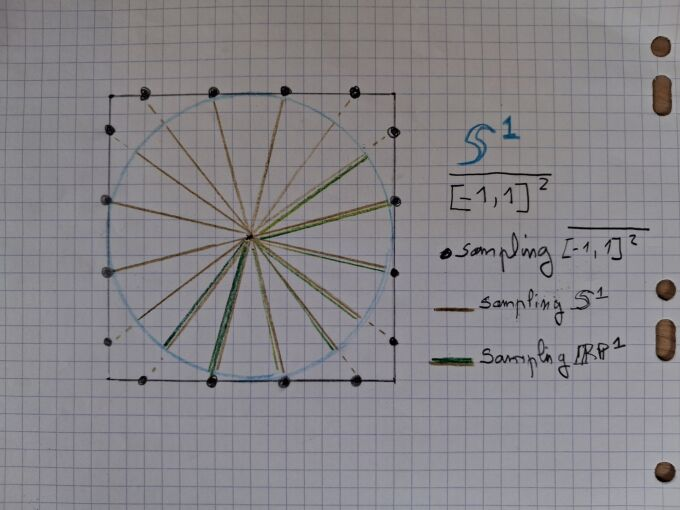
\includegraphics[width=8cm]{Programmer/ImagesProg/SamplSpher.jpg}
\caption{Illustration of sampling hypercube, sphere and projective sphere for $D=1$}
\label{fig:SamplSph:HeuristikOpt}
\end{figure}

We note $\Cub{N}$  the hypercube of $\RR^{N+1} $ the set of point $P$
such that $|P|_{\infty}=1$.  The mapping $\pi_{\infty/2} : P \rightarrow \frac{P}{|P|_2}$
is bijective continous between $\Cub{N}$ and $\SPH^N$
\footnote{the inverse maping being  $\pi_{2/\infty} : P \rightarrow \frac{P}{|P|_\infty}$},
so a reasonable way to sample $\SPH^N$ is to compute the image by $\pi_{\infty/2}$ of a sampling of 
$\Cub{N}$.

To sample $\Cub{N}$  we remark that it is made of $2*(N+1)$ faces, each one being 
homologous to ${[-1,1]^N}$.

Sometime we need to sample the projective hypercube, this mean  $\Cub{N}$ that 
is quotiented by relation $P \equiv -P$. In this case we must assure that we 
only get one of the two equivalent point , this is done taking the first $N+1$
face (it works because the order is adequate). 
Figure \ref{fig:SamplSph:HeuristikOpt} illustrate the sampling of $\SPH^1$, $\RP^1$ and $\Cub{1}$
with  $NbStep=4$.


\subsection{For the maintener of the code on hyper cube sampling}

We give some tricky detail on the implemantion.  To establish a mapping between numbers and point
of  $\Cub{N}$, we proceed this way :

\begin{itemize}
   \item let $K$ be a number;
   \item $F_K=\frac{K}{2(N+1)}$ will be the number of the face and $F^K = K\%(2(N+1)) $ the
         index inside the face ;
   \item  let $f$ be the number of points in each dimension and each face,  we make a $-adic$
          decomposition of  $F^k$ to have the coordinate the face.
\end{itemize}

This is implemented in the function {\tt cSampleHyperCube::KthPt}.

%----------------------------------------------------------------------------

\subsection{Programmer point of view for sampling the hyper cube}

The class {\tt cSampleHyperCube} allow to sample $\Cub{N}$,
this is \emph{non} template class, as is does not provide
{\tt cPtxd} but vectors.  This is rather an internal class
used for implemanting sampling of spheres.
The service offered are :

\begin{itemize}
   \item constructor {\tt cSampleHyperCube(int aDim,int aNbStep,bool isProj);}
         {\tt Dim} is the dimension,  {\tt aNbStep} indicate the number $f$
         of point in each dimension of each face 
         \footnote{there will bee $ 2* Dim * f^{Dim-1}$ sampled points},
         and {\tt isProj} indicate if it is the projective hypercube;

   \item accessor {\tt  int NbSamples() const;} indicate the number of sampled points;

   \item {\tt void  KthPt(std::vector<tREAL8> \& aPts,int aK) const;} put in vector
         {\tt aPts} the coordinates of $K^{th}$ point;

    \item accessor {\tt bool IsProj() const;} indicate if it is projective;
\end{itemize}

Enumerating all the sampled point, is done with a simple integer loop on
{\tt NbSamples} and acceding to sample with {\tt KthPt}.


%----------------------------------------------------------------------------
\subsection{Programmer point of view for sampling the sphere}
\label{HeurOpt:ProjSph}

\emph{For now only $\SPH^2$ is implemanted because that's what I needd, but a generic sampling 
of $SPH^N$ can easily be made using {\tt cSampleHyperCube} and taking example of {\tt cSampleSphere3D}}.

The class for sampling the sphere is {\tt cSampleSphere3D},  :


\begin{itemize}
   \item constructor {\tt cSampleSphere3D(int aNbStep,bool isProj)}, where {\tt NbStep} will
         be used by {\tt cSampleHyperCube} ;

   \item {\tt int NbSamples() const;} , {\tt cPt3dr KthPt(int aK) const;} {\tt bool IsProj() const;}
         quite obvious and similar to {\tt cSampleHyperCube} ;

    \item {\tt tREAL8  SqDist(const cPt3dr\& P1,const cPt3dr\& P2) const;} return the square
          distance between $P_1$ and $P_2$ taking into account the projective aspect of the sphere,
          it value $|P_1-P_2|^2$ if not projective, and $\min(|P_1-P_2|^2,|P_1+P_2|^2)$ in the
          projective case.
\end{itemize}


%----------------------------------------------------------------------------
\subsection{Sampling the space of rotations}

For sampling the space of rotation we use the quaternion and the well
known homeomorphism between $\RP^3$ and the space of rotation; the implemantion
use   {\tt cSampleHyperCube}  to sample $\Cub{3}$.

The class {\tt cSampleQuat} provide the service for sampling the quaternions :

\begin{itemize}
   \item {\tt cSampleQuat(int aNbElem,bool ForRot);} constructor, parameter have same meaning than 
         {\tt cSampleHyperCube}

   \item {\tt static cSampleQuat FromNbRot(int aNbRot,bool ForRot); } "static" constructor,
         instead of taking the number of step, take the total number of rotation required;

   \item {\tt size\_t NbRot() const;} number of rotation sampled;

   \item {\tt cPt4dr  KthQuat(int aK) const;}  return the $K^{th}$ quaternion, with $K<NbRot$;
   \item {\tt tRotR   KthRot(int aK) const;} transformate {\tt KthQuat} in rotation using {\tt Quat2MatrRot};
\end{itemize}


%----------------------------------------------------------------------------------------
%----------------------------------------------------------------------------------------
%----------------------------------------------------------------------------------------

\section{Global optimization on manifolds}

%----------------------------------------------------------------------------------------

\subsection{Introduction}

\label{HeurOpt:Man:Intro}

The need for optimization of a function on whole manifold comes originally from context where
we want to compute initial clinometer calibration from a set of measures.
In this context,  the calibration of a clino-meter is a unit vector, so a point of $\SPH^2$, and the criteria
the sum of residual that would be computed from a given calibration.  There is two main variant on
this basic case :

\begin{itemize}
   \item we can have $2$ clinometers that have been build to be almost orthogonal, and we want to enforce
         the orthogonality in the calibration;

   \item in some case, the verticalization can be approximative, or even the system can be totally not
         verticalized; 
\end{itemize}

If we take all the combination, we have $4$ possible cases :

\begin{itemize}
   \item if we have $1$ unknown clinometers $\vec I$ and the \emph{vertical is known}, we have an unkwon unit vector
          :   {\bf we optimize on $\SPH^2$};

   \item \emph{still with vertical known}, if we have $2$  clinometers $\vec I$ and $\vec J$ that 
         are forced to be orthogonal, then $\{\vec I,\vec J, \vec I \wedge \vec J\}$  is an orthonormal base, 
          that can be seen as a  rotation, {\bf we optimize on $\RP^3$}

   \item if we have $1$ clinometers  $\vec I$ and the \emph{vertical $\vec V$ is unknown}, 
         we have $2$ unkwon independant unit vector : {\bf we optimize on $\SPH^2 \times \SPH^2$} ; in 
         fact, as $\{\vec I,\vec V\}$ is not discernable from $\{-\vec I,-\vec V\}$ , 
          {\bf we can optimize on $\SPH^2 \times \RP^2$}
          
   \item if have $2$ ortognal clinometers  $\vec I,\vec J$ and the \emph{vertical $\vec V$ is unknown}, 
         we have an unknwon rotation and an unkown unit vector,  {\bf we optimize on $\RP^3 \times \SPH^2$};
         or if take into accound that  $\{\vec I,\vec J, \vec V\}$ and   $\{-\vec I,-\vec J, -\vec V\}$,
         {\bf we can optimize on $\RP^3 \times \RP^2$}.
\end{itemize}


To take into account all these configuration, and possibly new ones, and 
to avoid code duplication, the implementation that was done use template classes
that manipulates  manifolds descriptors. It also use a construction that allow to automatically
built the class correspond to $\MM_1 \times \MM_2$ from the classes describing
$\MM_1$ and $\MM_2$.

%----------------------------------------------------------------------------------------

\subsection{Methodology}

\subsubsection{Simple case}
The approach for optimization of a function $F$ on a manifold $\MM$  \emph{merge} the 
two methodologies seen in~\ref{HeurOpt:OBS} and~\ref{Sec:Samp:Sphere} :

\begin{itemize}
   \item  in a first step,  possible local extrema ${E_1,E_2 \dots}$ are extracted from the 
          sampling of $\MM$ using methods desribed on ~\ref{Sec:Samp:Sphere} ;

   \item  in a second step,  each $E_k$ is refined usign the methodology described in~\ref{HeurOpt:OBS} ;
          to explorate a neighoorhoud of $E_k$,  we will need to use  $\TgtM(E_k)$ ,
          a diffemorphism between a neighboorhoud of $E_k$ and a neighboorhoud of $0$ in $\RR^N$;
\end{itemize}

\subsubsection{Multiple extrema}
\label{HeurOpt:Man:MulrExtr}

In many case, extracting a single extrema on the sampling of $\MM$ is sufficient. By the way,
we have encountered cases where using a too rough sampling of $\MM$, the maxima extracted is
not close to the global maxima. So for computing multiple maxima we process this way :

\begin{itemize}
   \item start we the global maxima $E_1$;
    \item each time a new maxima $E_k$ is found, mark as reached all the point of the sampling
          such as $D_{\MM}(P,E_k) < \delta$  where $\delta$ is a threshold, where $D_{\MM}$ is
          the distance on the manifold.
\end{itemize}

%----------------------------------------------------------------------------------------

\subsection{Maintener's point of view, requirement for class describing a Manifold}

\label{HeurOpt:ClassDescMan}

We describe here the requirement that a class must comply with to a descriptor of
manifold~\footnote{typicall the concept of \CPP20 may be adapted to describe this}.
Note that most current manifold being described, for the user it's not mandatory 
to see in detail this section.


Maybe the simpler way is to take an example, we will use the case of $\SPH^2$ 
implemanted in the class {\tt cSph3\_OptimDisc}. The class must contains :

\begin{itemize}
    \item {\tt        typedef cPt3dr tObj;} the type of the object contains in the manifold;

    \item {\tt static constexpr int DimTgtSp =2;}   a number indicate the dimension of tangent space  

    \item {\tt  typedef cP3dNormWithUK  tDescrTgtSp;}  a descriptor of tangent space, i.e. 
          the type of data that will be used to computed  $\TgtM(E_k)$; in this case, we use
          the type {\tt cP3dNormWithUK} that already exist because it contains the tangent space;


    \item {\tt  typedef cPtxd<tREAL8,DimTgtSp> tPtTgt;} not a requirement, but convenient;


    \item {\tt int NbObjDisc() const ;} a method indicating the  number of sampled point;

    \item {\tt   tObj KthObjDisc(size\_t aK) const;} a method returing the  $K^{th}$ sample;

    \item   {\tt  tREAL8 SqDist(const tObj \& aP1,const tObj \& aP2) const} a method returning
          the square distance between $2$ points, in this case the method will take into account
          the possible projective aspect of the sphere;


    \item   {\tt   tREAL8 Density();} a method return a (very) approximative estimator of the density;

    \item   {\tt   tDescrTgtSp * CreateTgtSpace(const tObj \& aPt) const;} a method indicating
           how to compute  {\tt tDescrTgtSp*} in a given point;

    \item   {\tt          void DeleteObjFromTgtSp(tDescrTgtSp * anObj) const;} a method
            for freeing memory (because {\tt delete} will not always work);

    \item   {\tt  tObj GetObjFromTgSpace(const tDescrTgtSp \& aP3N, const tPtTgt\& aPTgt) ; } a method
             implementing the $\TgtM(E_k)$ ;

\end{itemize}

The class implementing the manifold of rotation is even simpler, because the descriptor
of tangent space, is simply the rotation themselves.

%----------------------------------------------------------------------------------------

\subsection{Cartesian product of manifolds}

We have seen bellow, that it often happen that we need to make an optimization
of $\MM_1 \times \MM_2$ where $\MM_1$ and $\MM_2$ are two manifolds. For
this, we can use  the class {\tt cCartProduct\_OptimDisc<T1,T2>} :

\begin{itemize}
    \item if {\tt T1} and {\tt T2} are two classes that comply with requirement
          of~\ref{HeurOpt:ClassDescMan} for describing the manifolds $\MM_1$ and $\MM_2$ ;
    \item the {\tt CartProduct\_OptimDisc<T1,T2>} will be class for describing
           $\MM_1 \times \MM_2$;
    \item  \emph{hopefully}, \footnote{not tested \dots}  {\tt CartProduct\_OptimDisc<T1,T2>} 
           complies with~\ref{HeurOpt:ClassDescMan} and iterating the construction can
           be used to create descriptors of $\MM_1 \times \MM_2 \times \MM_3$ \dots
\end{itemize}

Note the definition
{\tt typedef cCartProduct\_OptimDisc<cSph3\_OptimDisc,cRot\_OptimDisc>  tPoseCart\_OptimDisc;},
that construct a decriptor of the manifold of poses : a pose being the concatenation of a unit
vector and a rotation. And there is a facilty for construction it :

\begin{itemize}
  \item {\tt inline tPoseCart\_OptimDisc  Pose\_OptimDisc(int aNbTr,bool isSPhProj,int aNbRot)} 

  \item with {\tt NbTr} and {\tt NbRot} indicating the number of discrtization on translation and rotation


  \item with {\tt isSPhProj} indicating if sphere is projective ; {\tt true} for clino calibration
          as desrcibed in~\ref{HeurOpt:Man:Intro} ; {\tt false} if used in pose estimation.
\end{itemize}


%----------------------------------------------------------------------------------------

\subsection{User's point of view}

Once the manifold descriptor have been build, the class {\tt cTplOptDisc\_OnManifold}
can be used to optimize a function on manifold. The method are :

\begin{itemize}
   \item the constructor that take in parameter the descriptor of manifold and 
         the function to minimize as a {\tt cOptDiscScorer<tObj>};

   \item  {\tt void ComputeSol ( tREAL8 aDistNeigh, tREAL8 anEpsilon, int aNbTest)}
           compute the solution, {\tt aDistNeigh} and  {\tt aNbTest} are used to compute
          the multiple extrema as described in~\ref{HeurOpt:Man:MulrExtr}
   \item  {\tt GetSol} give access to extrema, once {\tt ComputeSol} was called;
\end{itemize}









